\chapter{Graphical Interface and Application Execution}
\label{chap:ch4}

\tolerance=9999
\emergencystretch=3em

\indent \par Chapter \ref{chap:ch3} described how the system was built. This chapter describes how it actually looks and behaves once it is running. The discussion is split in three parts. The first part presents the graphical interface as a whole, screen by screen, so the reader can map the abstract components from the previous chapter to the actual buttons and panels he would see on his own machine. The second part is a mini walkthrough of the main functionality, peer-assisted streaming, as a user would experience it from the home screen up to the statistics view. The third part consolidates the steps into a short user manual.

\par Throughout the chapter, the screenshots are taken from the macOS build of the application, with a small library imported from disk and a single user signed in. The authentication flow itself is documented in Section \ref{subsec:auth} of the previous chapter and does not have its own screenshot here. All the screens have a persistent navigation drawer on the left and a persistent player bar at the bottom; the middle area is what changes when the user moves between sections.


\section{The Graphical Interface}
\label{sec:gui}

\subsection{Home and Main Scaffold}
\label{subsec:gui-home}

\indent \par Figure \ref{fig:screen-home} shows the home screen, which is the first screen the user sees after the bootstrap completes. The left drawer lists the seven destinations of the application: Home, Albums, Artists, Music (the tracks list), Playlists, Upload songs and Statistics. The user settings entry is at the bottom of the drawer, and shows the email of the currently signed-in user.

\par The middle area of the home screen is composed of three horizontal rails: ``Jump back in'' with the recently played albums, ``Recommended for you'' with suggestions based on the listening history, and ``Rediscover'' with songs that the user has not listened to in a while. Each card displays the cover art, the title and the artist name. The persistent player bar at the bottom shows the currently playing song, the lyrics line at the centre, and the playback controls on the right (shuffle, previous, play/pause, next, repeat, and expand).

\begin{figure}[htbp]
\centering
\includegraphics[width=\textwidth]{figures/screenshots/home_screen.png}
\caption{Home screen with the navigation drawer, the three home rails (jump back in, recommended, rediscover), and the persistent player bar.}
\label{fig:screen-home}
\end{figure}

\subsection{Browsing the Catalogue}
\label{subsec:gui-catalogue}

\indent \par The catalogue can be browsed in three different ways, depending on what the user is looking for. The Music entry in the drawer opens the tracks view, shown in Figure \ref{fig:screen-tracks}. Songs are laid out as a grid of cover art with the title underneath; a search bar at the top filters by track name and the icons in the top right control sorting and shuffling.

\begin{figure}[htbp]
\centering
\includegraphics[width=\textwidth]{figures/screenshots/tracks_screen.png}
\caption{Tracks view, opened from the Music entry in the drawer. The grid is filterable through the search bar and sortable through the controls in the top right.}
\label{fig:screen-tracks}
\end{figure}

\par The Albums and Artists entries open similar grid views, focused on albums and on artists respectively. Figure \ref{fig:screen-albums} shows the albums view and Figure \ref{fig:screen-artists} the artists view. Selecting an album opens its detail page with the track listing; selecting an artist opens its detail page with both the artist's albums and his songs.

\begin{figure}[htbp]
\centering
\includegraphics[width=\textwidth]{figures/screenshots/albums_screen.png}
\caption{Albums view.}
\label{fig:screen-albums}
\end{figure}

\begin{figure}[htbp]
\centering
\includegraphics[width=\textwidth]{figures/screenshots/artists_screen.png}
\caption{Artists view.}
\label{fig:screen-artists}
\end{figure}

\subsection{Playlists}
\label{subsec:gui-playlists}

\indent \par The Playlists entry in the drawer opens the playlists view, depicted in Figure \ref{fig:screen-playlists}. The user can create new playlists, rename them, and reorder the songs inside. The built-in ``Liked Songs'' playlist is always present, marked indestructible at the database level (see Section \ref{subsec:schema-user}) so that it cannot be deleted by accident.

\begin{figure}[htbp]
\centering
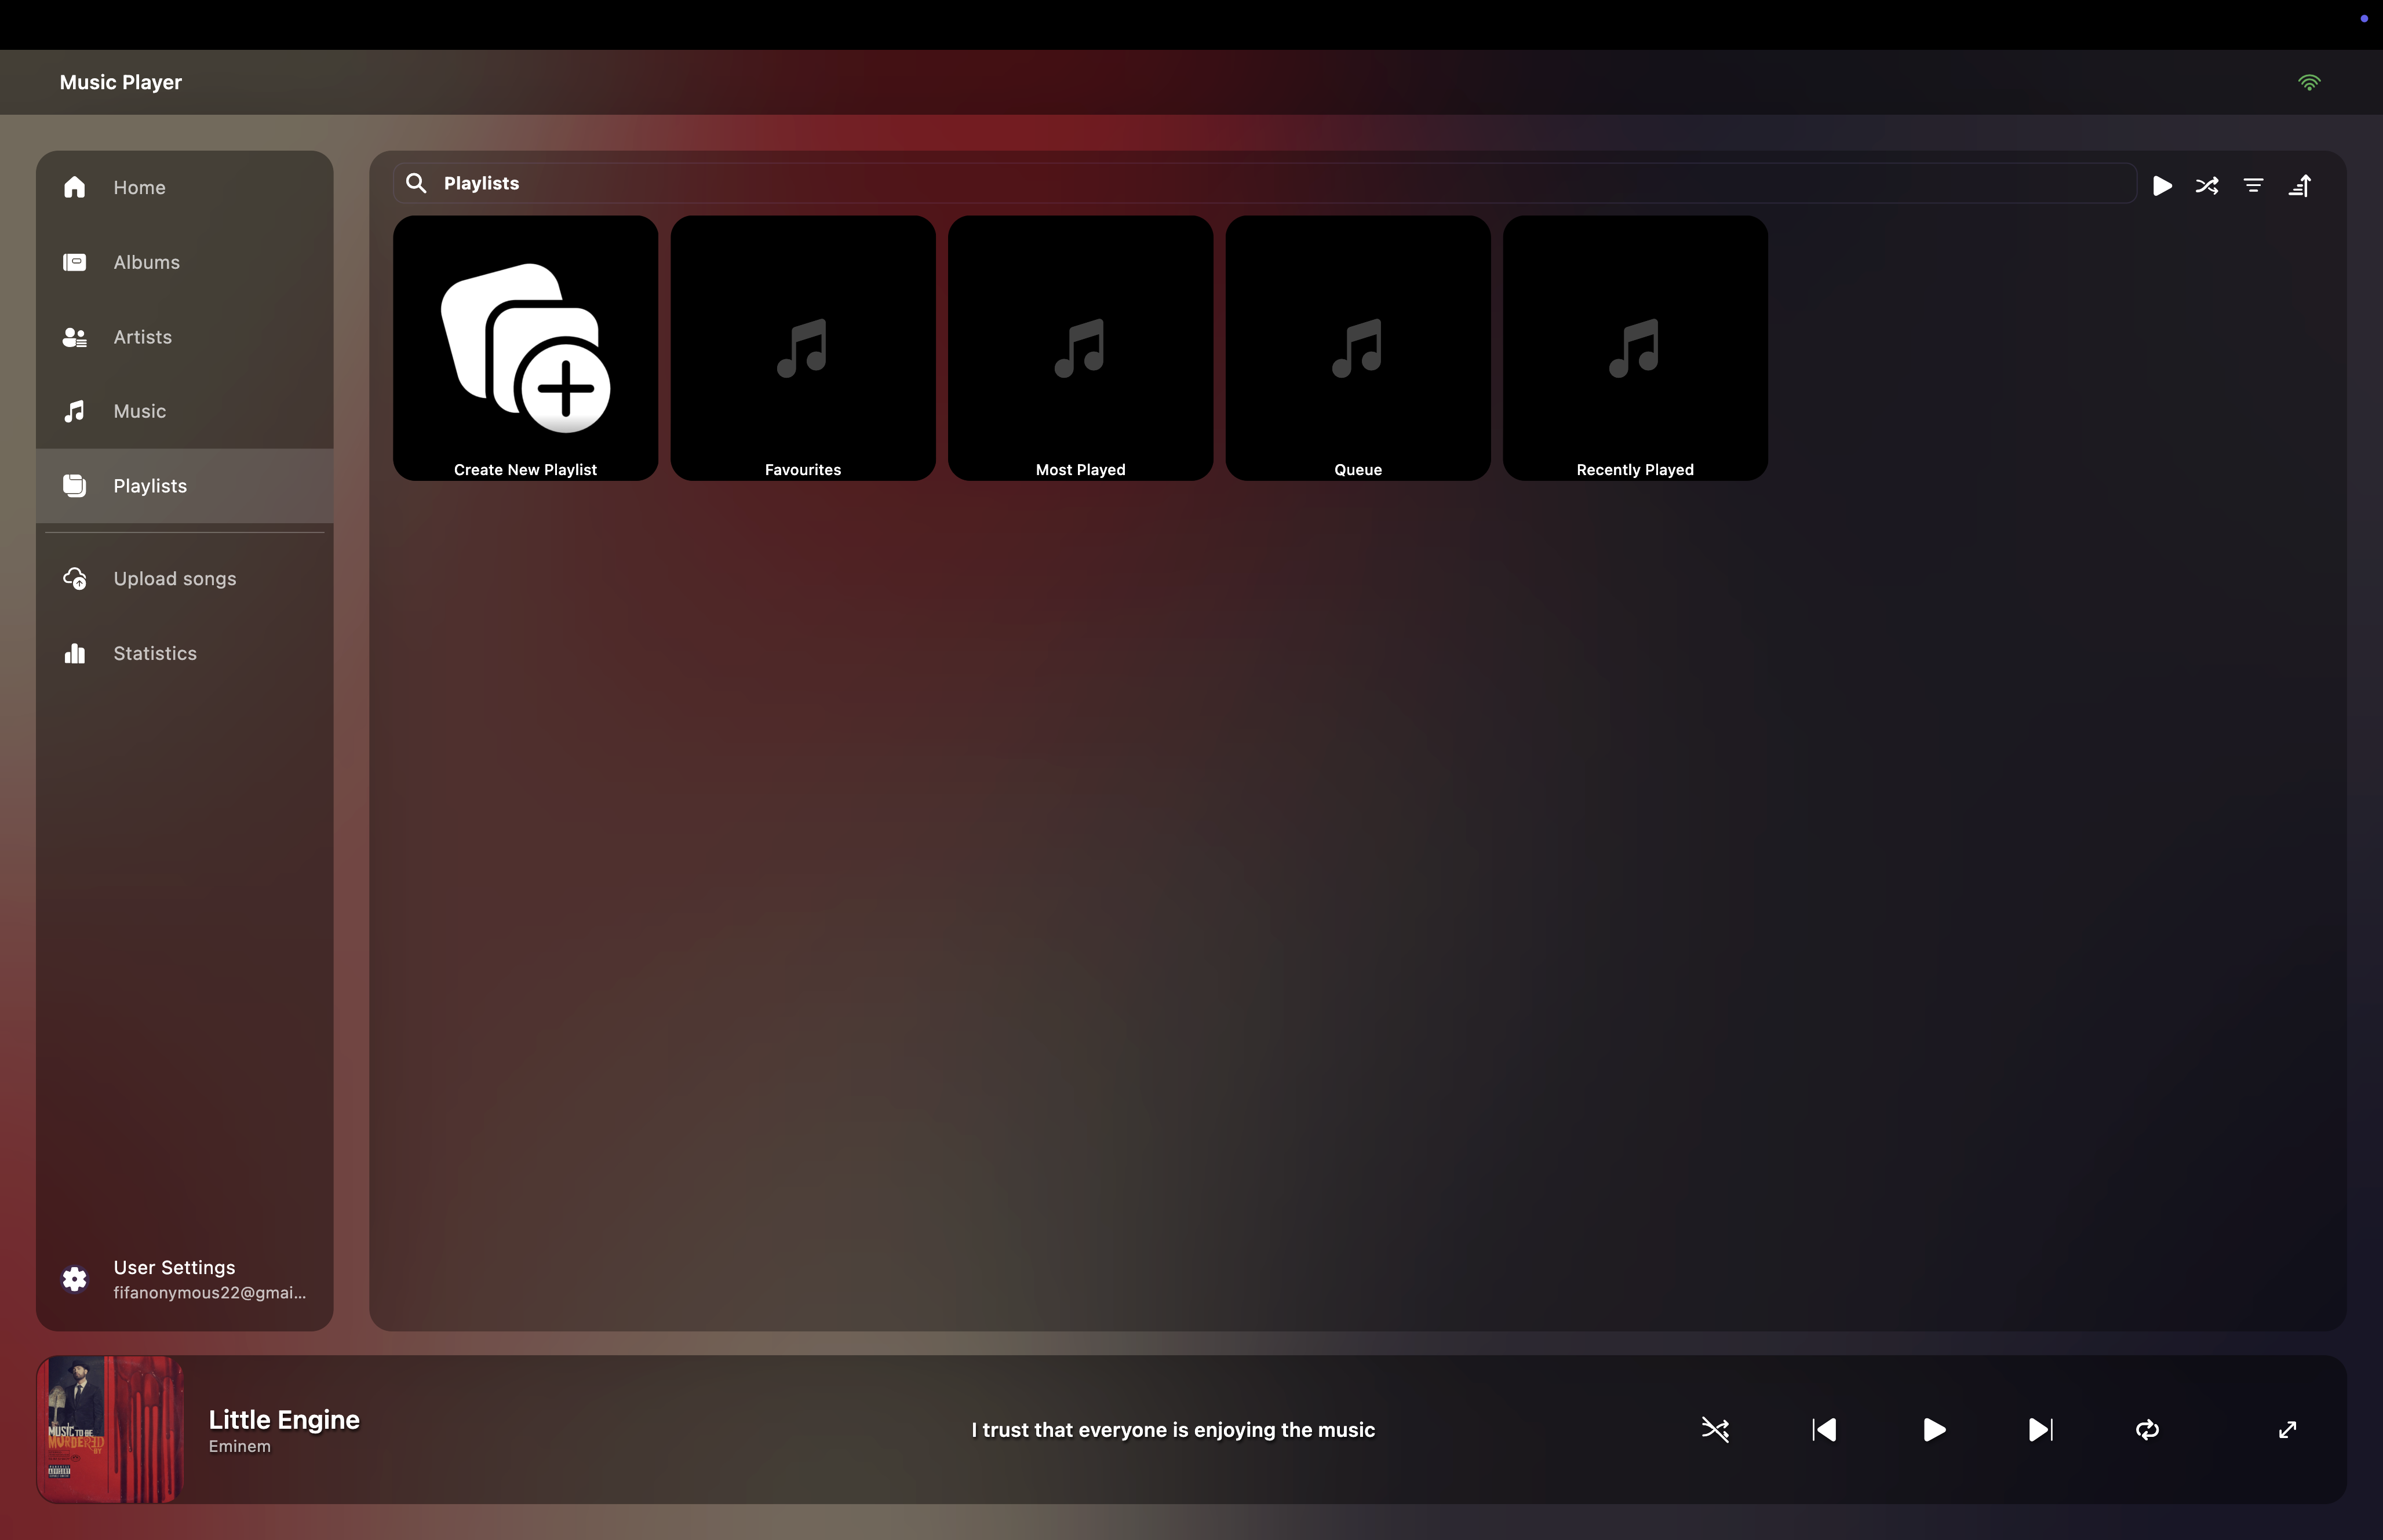
\includegraphics[width=\textwidth]{figures/screenshots/playlists_screen.png}
\caption{Playlists view.}
\label{fig:screen-playlists}
\end{figure}

\subsection{Now Playing}
\label{subsec:gui-now-playing}

\indent \par Tapping on the player bar at the bottom of the scaffold expands it into the now playing screen, shown in Figure \ref{fig:screen-now-playing}. The middle section displays the cover art of the currently playing song; the left side shows the lyrics, when available, scrolled along the playback position; the right side shows the upcoming queue. A heart icon on the cover toggles the liked state, which fires a \texttt{PATCH /songs/\{fileHash\}} request as described in Section \ref{subsec:state-sync}. The progress bar and the standard playback controls run along the bottom.

\begin{figure}[htbp]
\centering
\includegraphics[width=\textwidth]{figures/screenshots/expanded_music_player_widget.png}
\caption{Expanded now playing screen with the lyrics on the left, the cover in the centre, and the queue on the right.}
\label{fig:screen-now-playing}
\end{figure}

\subsection{Uploading Songs}
\label{subsec:gui-upload}

\indent \par The Upload songs entry in the drawer opens the upload screen, shown empty in Figure \ref{fig:screen-upload-empty}. The user selects one or more audio files from disk; each file is added to the upload list and shown with its title and artist as parsed from the file's metadata, as in Figure \ref{fig:screen-upload-song}. Pressing the Upload button runs the negotiated upload protocol from Section \ref{subsec:upload}: the client first calls \texttt{POST /songs/negotiate} with the manifest of chunk hashes, and then sends only the missing chunks through \texttt{POST /songs/\{fileHash\}/chunks/\{chunkIndex\}}.

\begin{figure}[htbp]
\centering
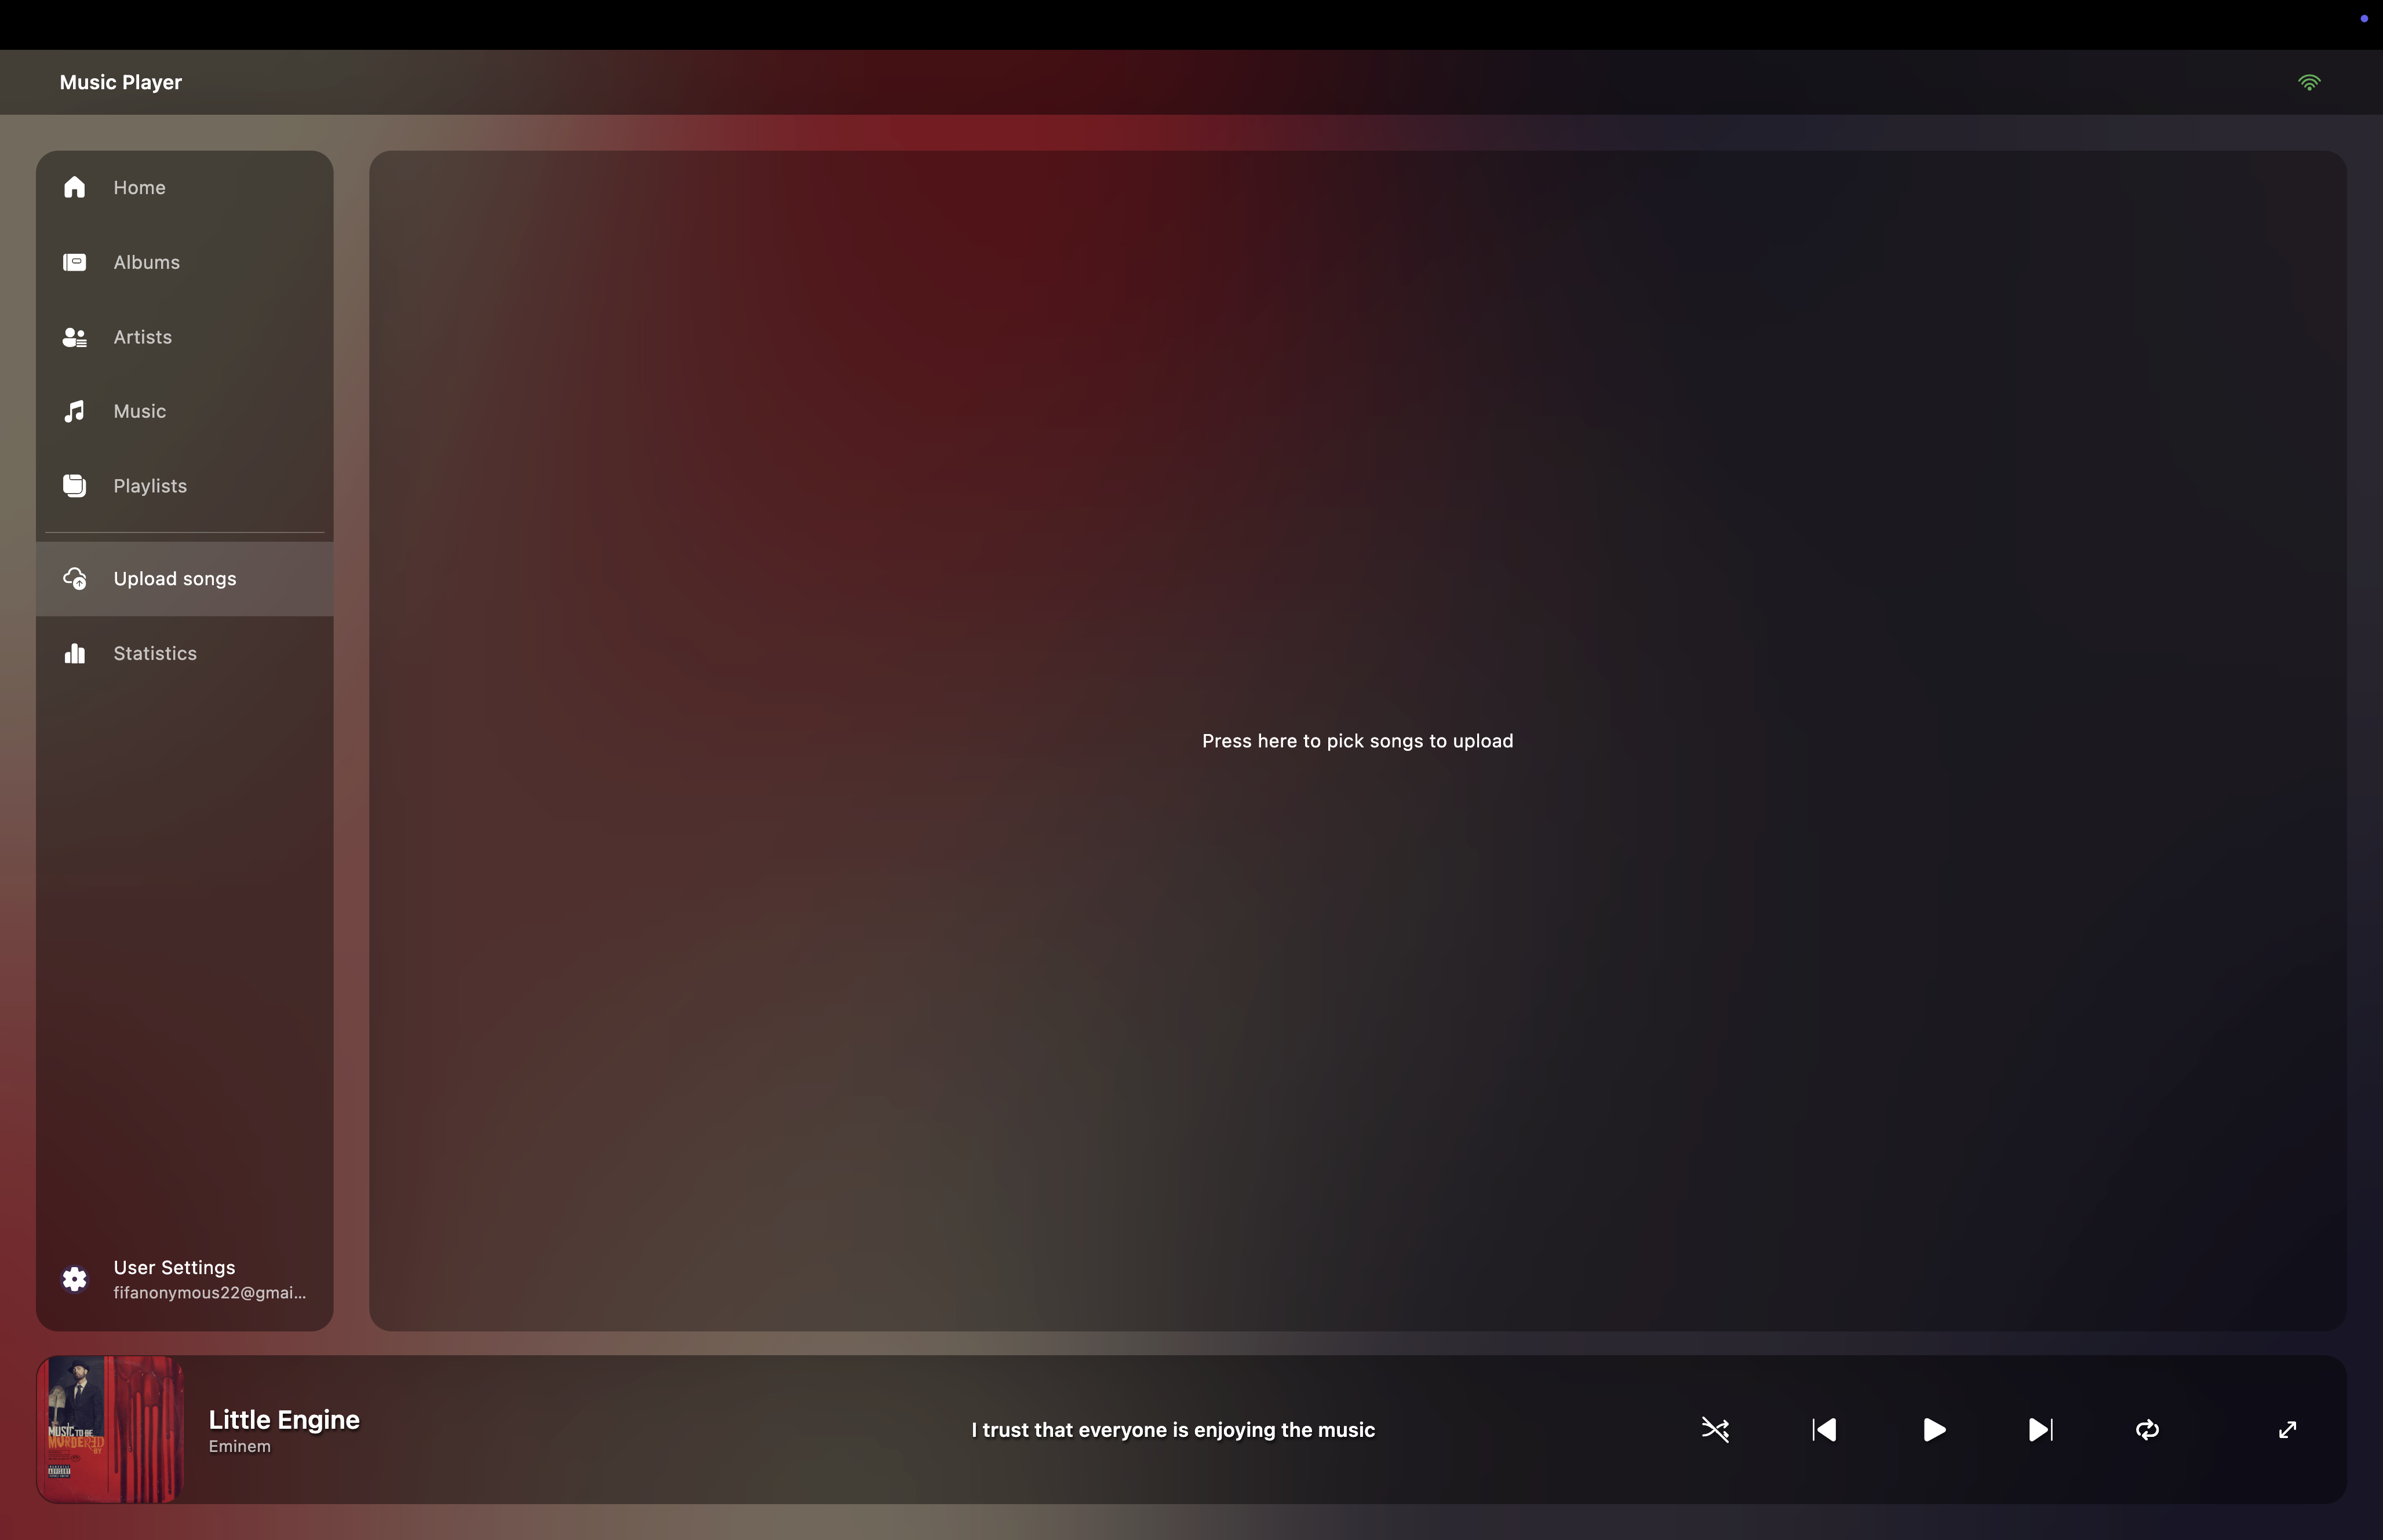
\includegraphics[width=\textwidth]{figures/screenshots/upload_screen_empty.png}
\caption{Upload screen, empty. The placeholder invites the user to pick songs from disk.}
\label{fig:screen-upload-empty}
\end{figure}

\begin{figure}[htbp]
\centering
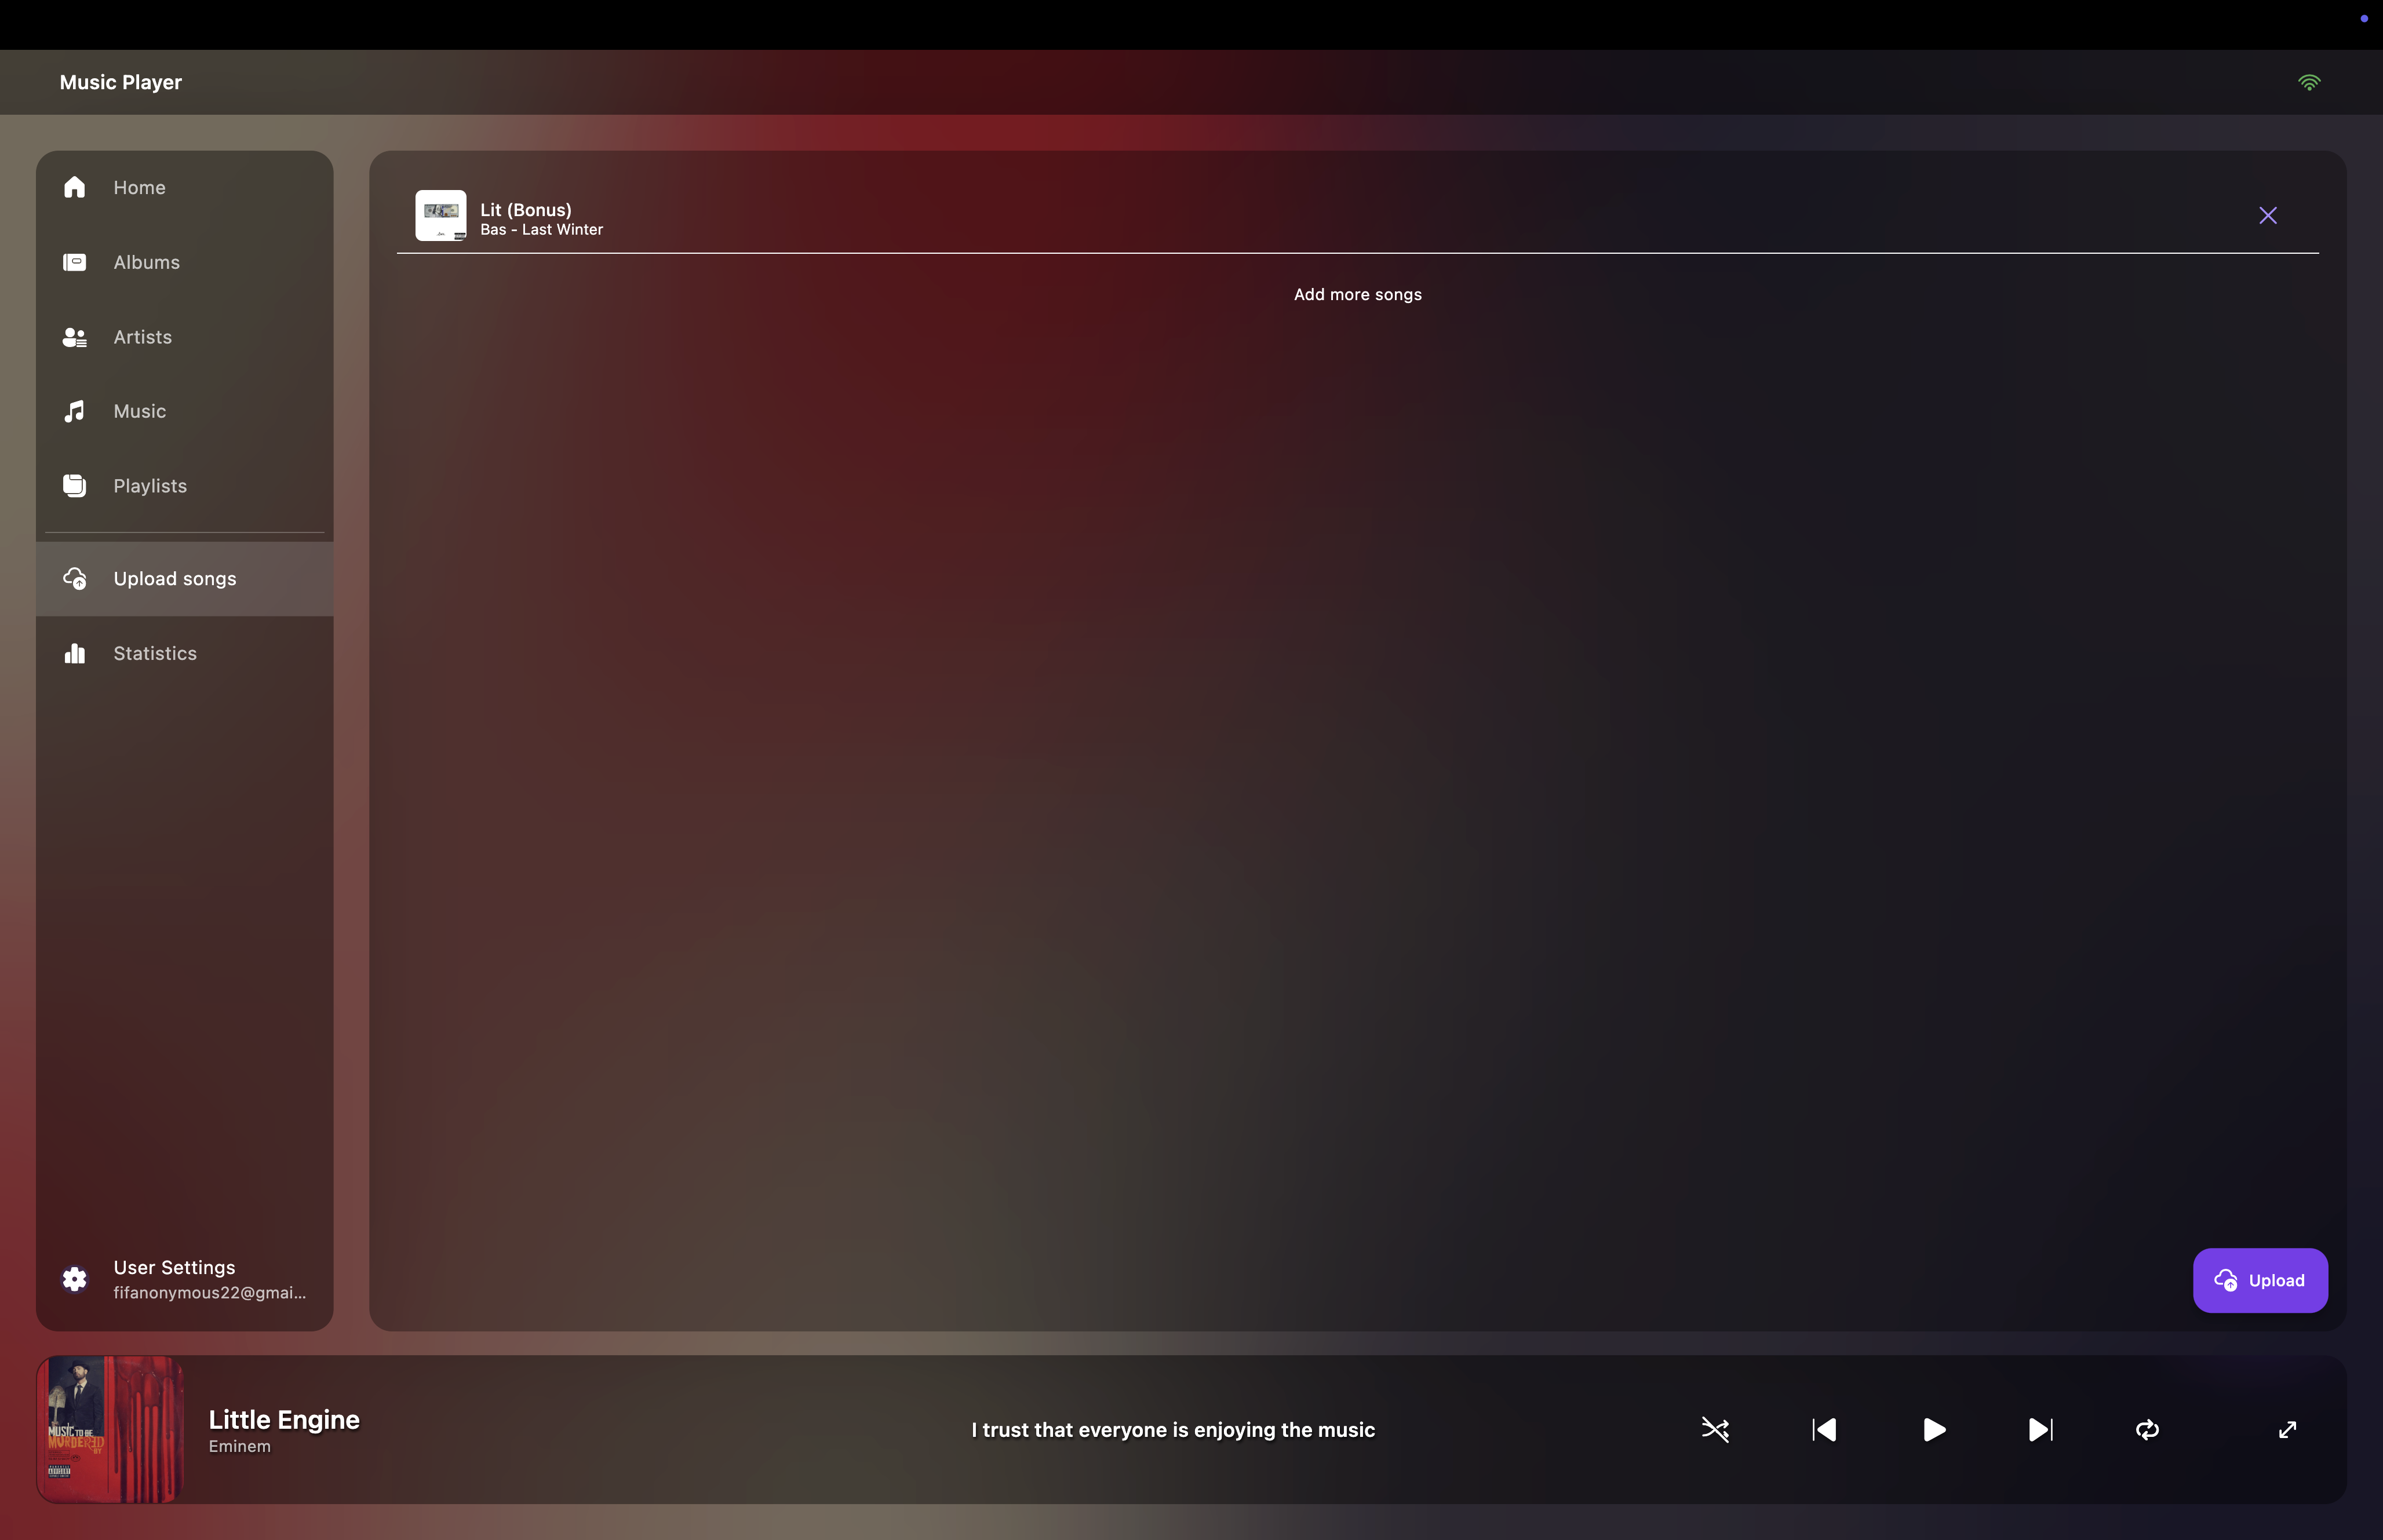
\includegraphics[width=\textwidth]{figures/screenshots/upload_screen_song.png}
\caption{Upload screen with one song queued, ready to be sent through the negotiated upload protocol.}
\label{fig:screen-upload-song}
\end{figure}

\subsection{Settings}
\label{subsec:gui-settings}

\indent \par The User Settings entry at the bottom of the drawer opens the settings screen, shown in Figure \ref{fig:screen-settings}. The exposed options are kept intentionally short. The Account row shows the signed-in user and a Logout button. The Playback Speed slider sets the global playback rate. The Peer Network dropdown selects the connection types on which the application is allowed to act as a peer (Wi-Fi only, Cellular only, or both), as described in Section \ref{subsec:upload-limits}. The WiFi Data Limit and Cellular Data Limit sliders set the monthly upload caps for each type of connection.

\begin{figure}[htbp]
\centering
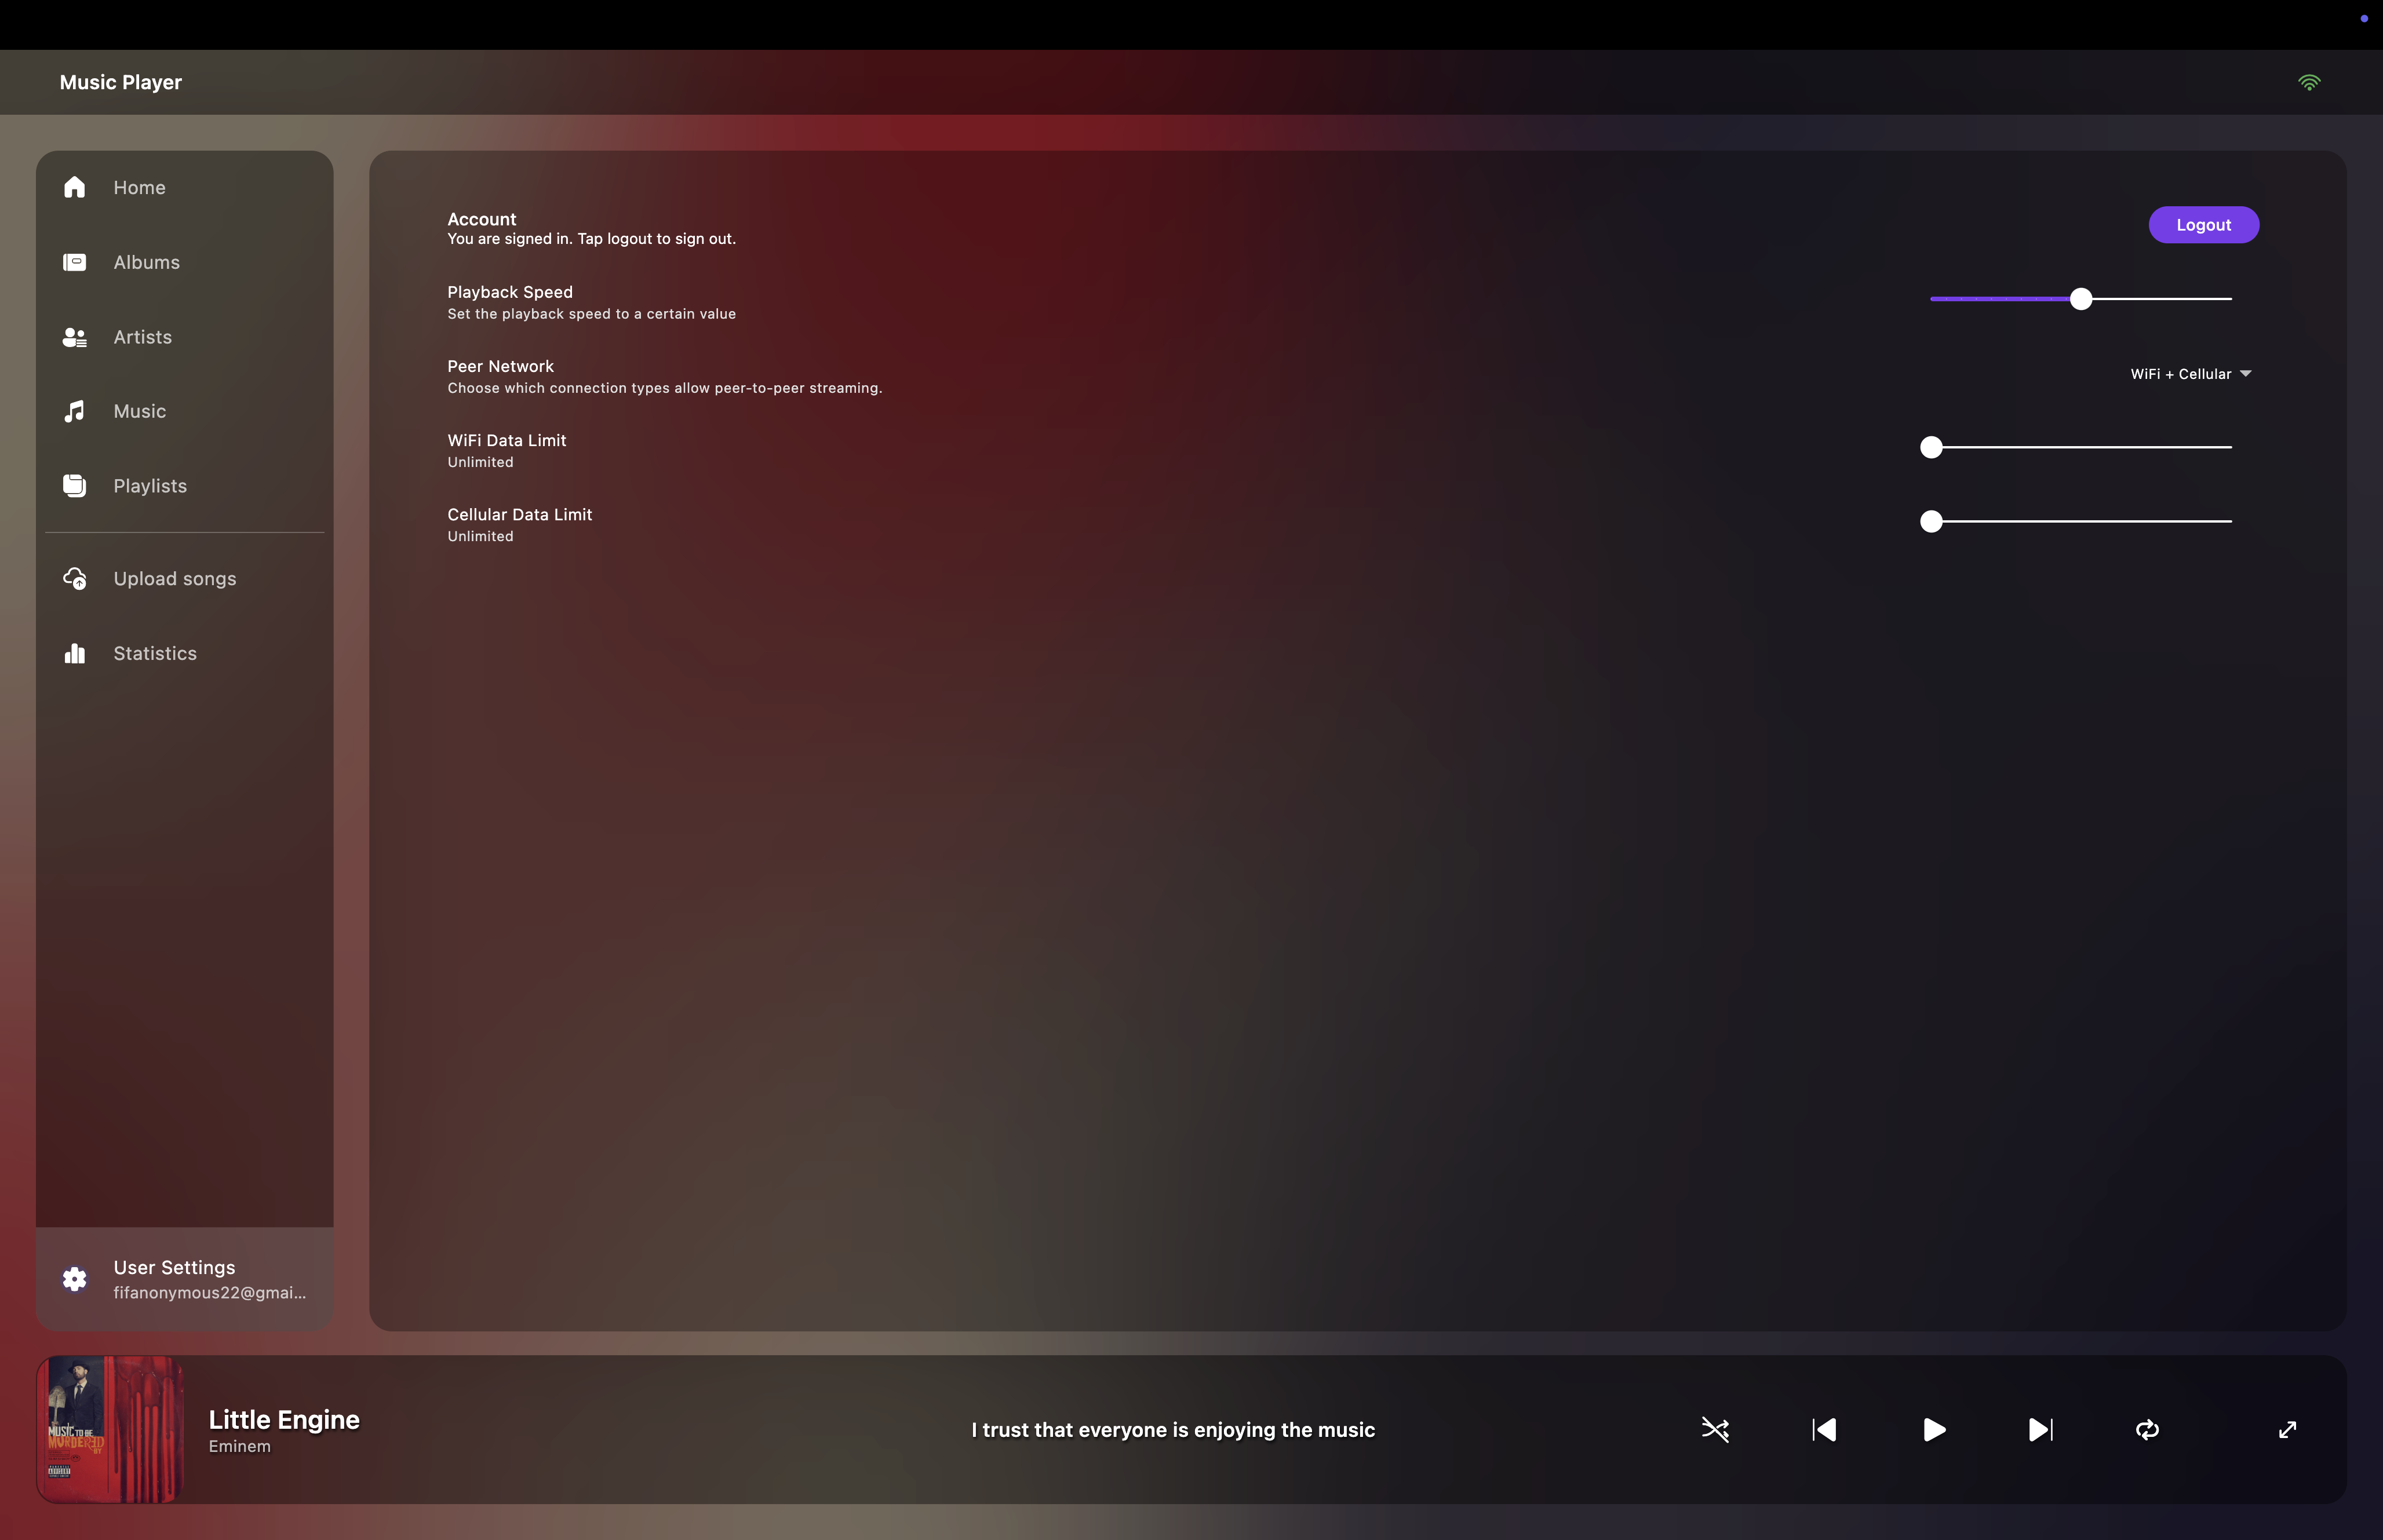
\includegraphics[width=\textwidth]{figures/screenshots/settings_screen.png}
\caption{Settings screen, with the account, the playback speed, and the peer network options.}
\label{fig:screen-settings}
\end{figure}

\subsection{Statistics}
\label{subsec:gui-stats}

\indent \par The Statistics entry in the drawer opens the screen shown in Figure \ref{fig:screen-stats}, which is the user-visible representation of the \texttt{chunk\_stats} rows described in Section \ref{subsec:schema-aux}. The card at the top aggregates the entire history: the average P2P share, the cumulative number of P2P chunks, the cached chunks, the local files, and the total chunks ever served. Below the card, every recorded session is shown as its own row, with the song name, the per-session P2P percentage on the right, the source breakdown (server/peer/local) underneath the title, and the timestamp on the bottom right.

\begin{figure}[htbp]
\centering
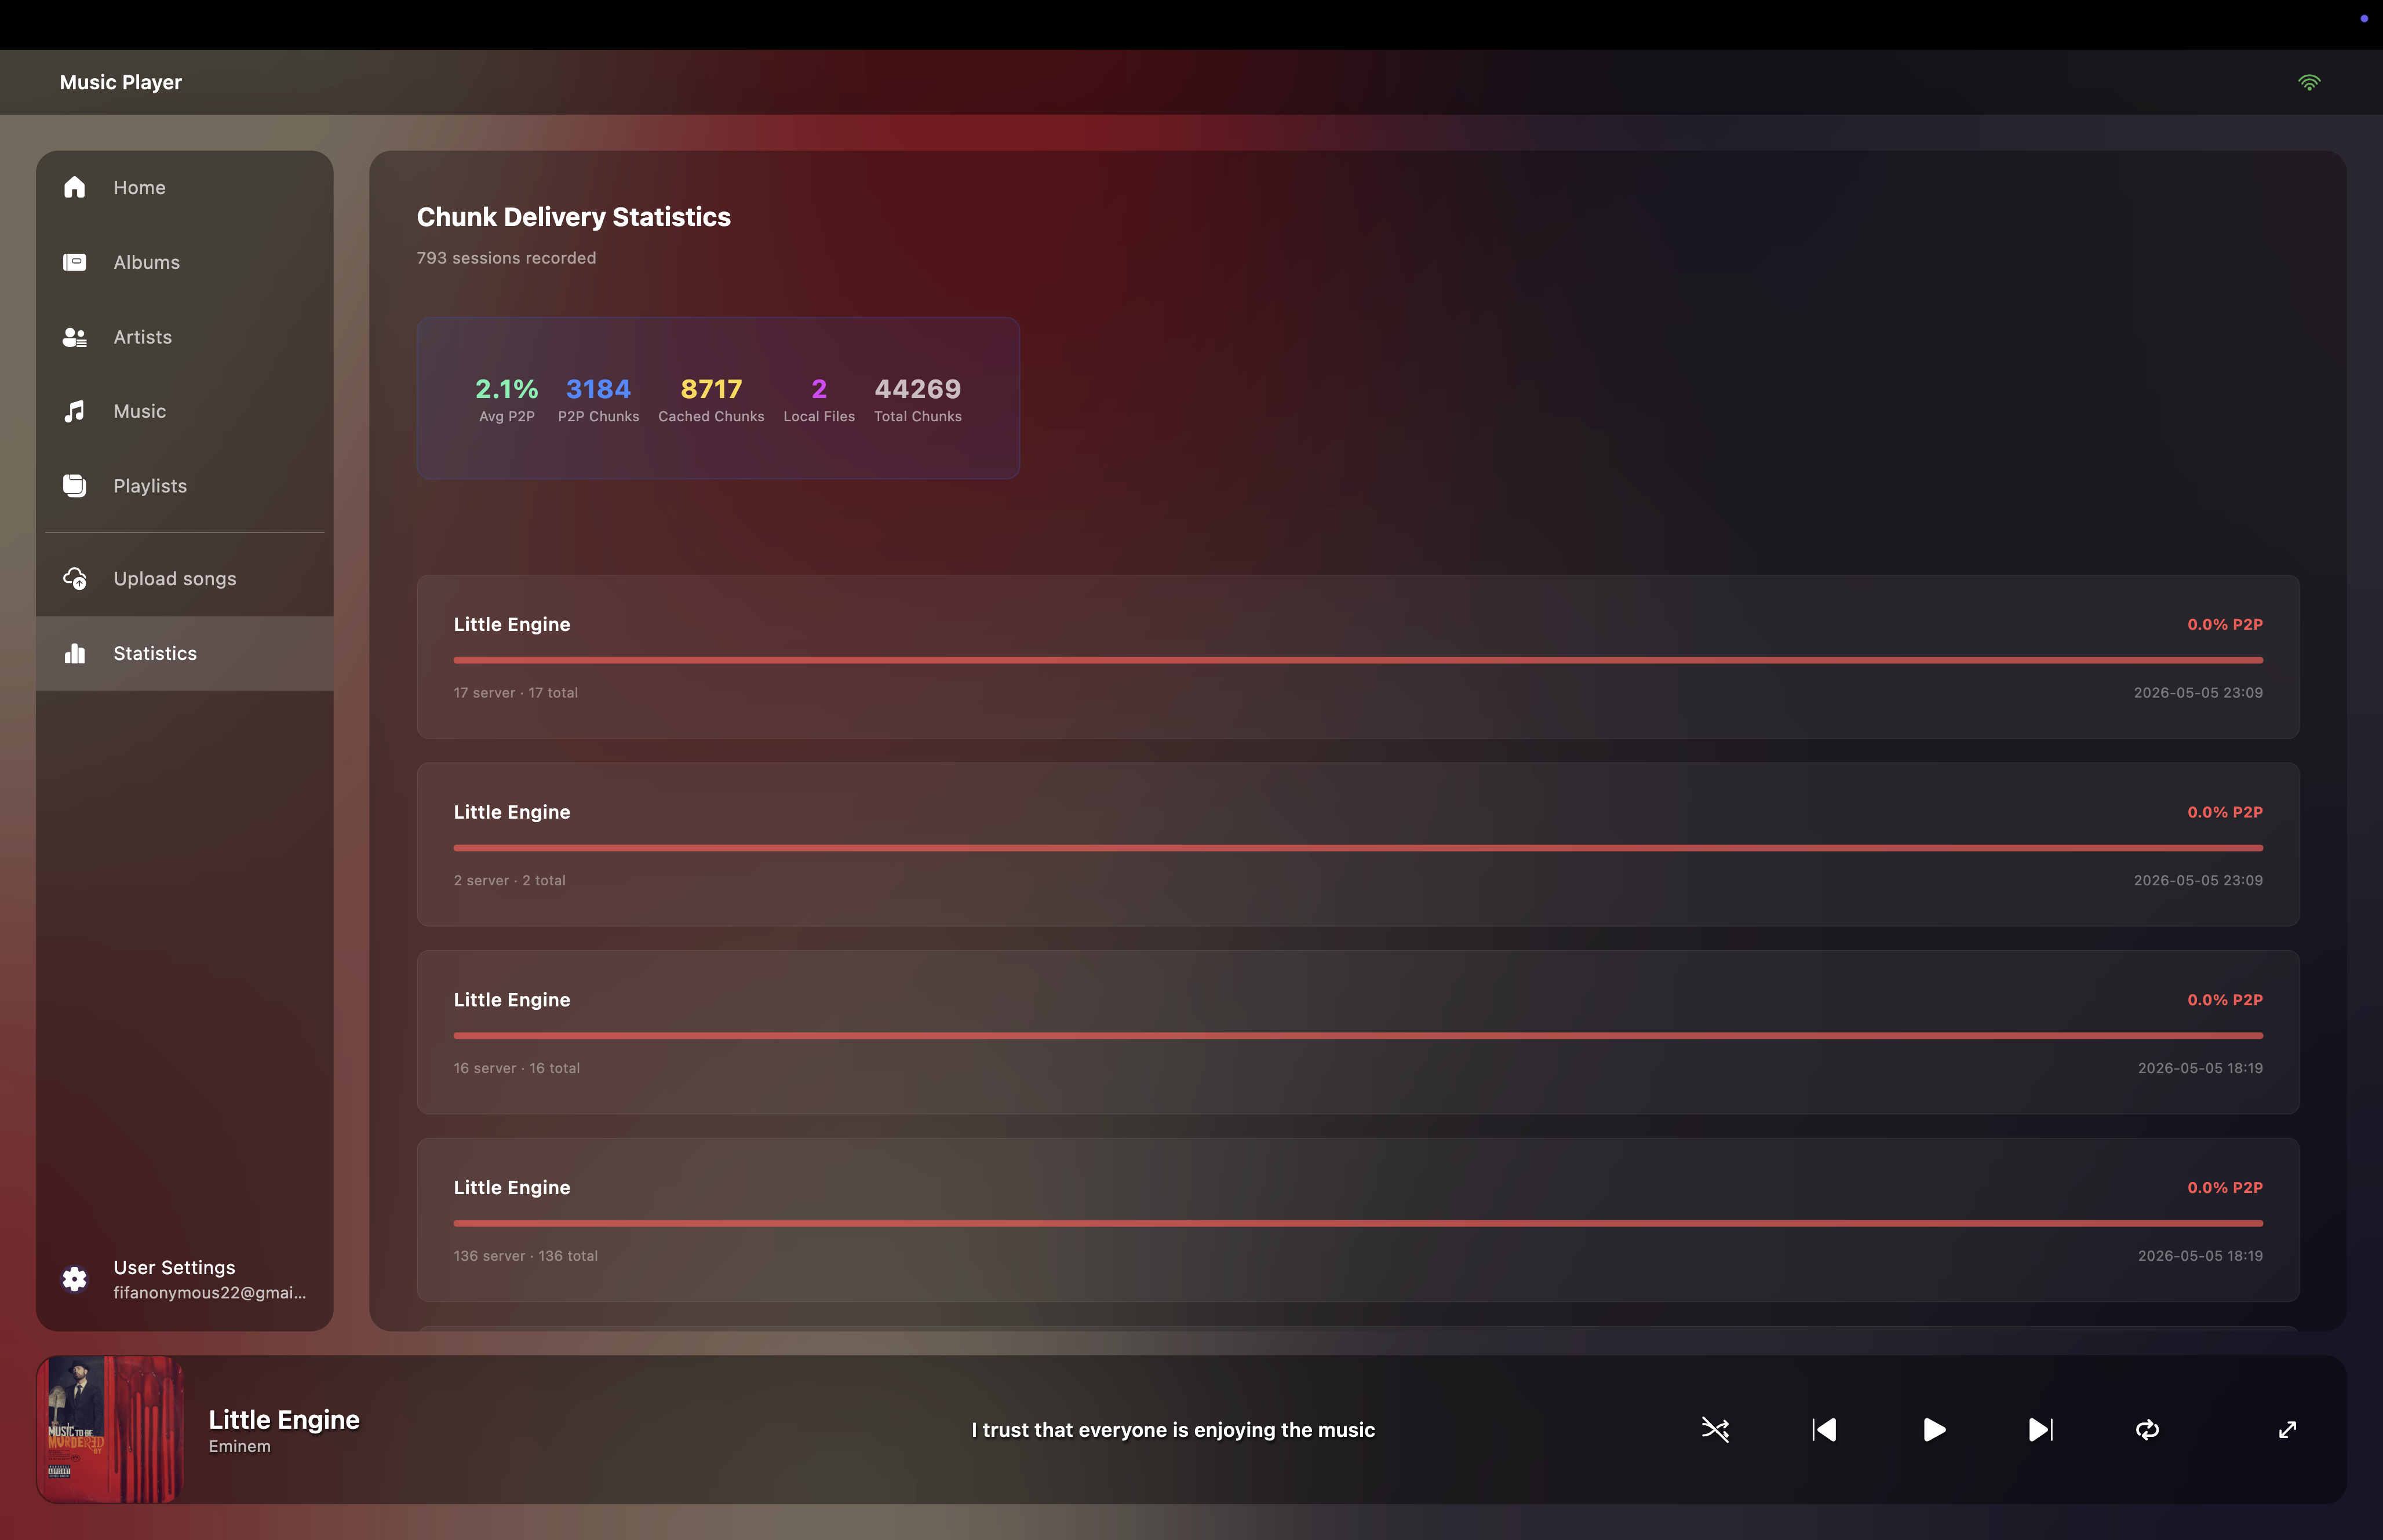
\includegraphics[width=\textwidth]{figures/screenshots/stats_screen.png}
\caption{Statistics screen with the aggregate card at the top and the per-session rows below.}
\label{fig:screen-stats}
\end{figure}


\section{Application Execution: Peer-Assisted Streaming}
\label{sec:exec-f1}

\indent \par This section walks through the main functionality of the application, the peer-assisted streaming, as a user would experience it from sign-in to verification. Each step below corresponds to one screenshot and to one observable effect on the system.

\subsection{Step 1: Reaching the Home Screen}
\label{subsec:exec-home}

\indent \par After the bootstrap completes (Sections \ref{sec:bootstrap}), the user lands on the home screen reproduced in Figure \ref{fig:exec-home}. At this point, the signaling WebSocket is already open, the access token has been refreshed, and the playback state has been pulled from \texttt{GET /playback}. The home rails are filled in from the recently played, recommended and rediscover endpoints, all of which read from the user library table.

\begin{figure}[htbp]
\centering
\includegraphics[width=\textwidth]{figures/screenshots/home_screen.png}
\caption{Home screen reached after the bootstrap completes, with the persistent player bar still showing the previously played song.}
\label{fig:exec-home}
\end{figure}

\subsection{Step 2: Selecting a Song}
\label{subsec:exec-select}

\indent \par From the drawer, the user opens the Music entry to reach the tracks view (Figure \ref{fig:exec-tracks}) and clicks on a song. The application calls \texttt{setQueueAndPlay} on the audio service, which builds the audio source and asks the chunk service for the manifest. On the first byte-range request, the service issues \texttt{GET /stream/\{fileHash\}/manifest} and, in parallel, \texttt{DISCOVER\_PEERS} over the signaling socket.

\begin{figure}[htbp]
\centering
\includegraphics[width=\textwidth]{figures/screenshots/tracks_screen.png}
\caption{Tracks view from which the user picks the song to play.}
\label{fig:exec-tracks}
\end{figure}

\subsection{Step 3: Playback Active}
\label{subsec:exec-playing}

\indent \par Tapping on the player bar expands it to the now playing screen, shown in Figure \ref{fig:exec-now-playing}. The first chunks (the 5\% prefix from equation \eqref{eq:prefix-impl}) are served by the origin server while the WebRTC handshake completes in the background. Once the data channel with the peer is open, the chunks above the prefix threshold are pulled directly from the peer; any peer timeout falls back transparently to the server, with the buffer absorbing the latency. The user sees only the smoothly advancing progress bar.

\begin{figure}[htbp]
\centering
\includegraphics[width=\textwidth]{figures/screenshots/expanded_music_player_widget.png}
\caption{Now playing screen during peer-assisted playback. The cover art, the lyrics, the queue and the progress bar are visible.}
\label{fig:exec-now-playing}
\end{figure}

\subsection{Step 4: Verifying Delivery on the Statistics Screen}
\label{subsec:exec-stats}

\indent \par When the song ends, or every 15 seconds during playback, the chunk service posts the cumulative counters to \texttt{POST /statistics}. To verify the result, the user opens the Statistics entry in the drawer, which produces the screen shown in Figure \ref{fig:exec-stats}. The aggregate card shows that, across all 793 sessions recorded so far, the application served on average 2.1\% of the bytes through peers, with the rest coming from the local cache (the dominant source in this single-user development setup) and from the origin server. The per-session list below the card breaks down each play and shows when peers were involved.

\begin{figure}[htbp]
\centering
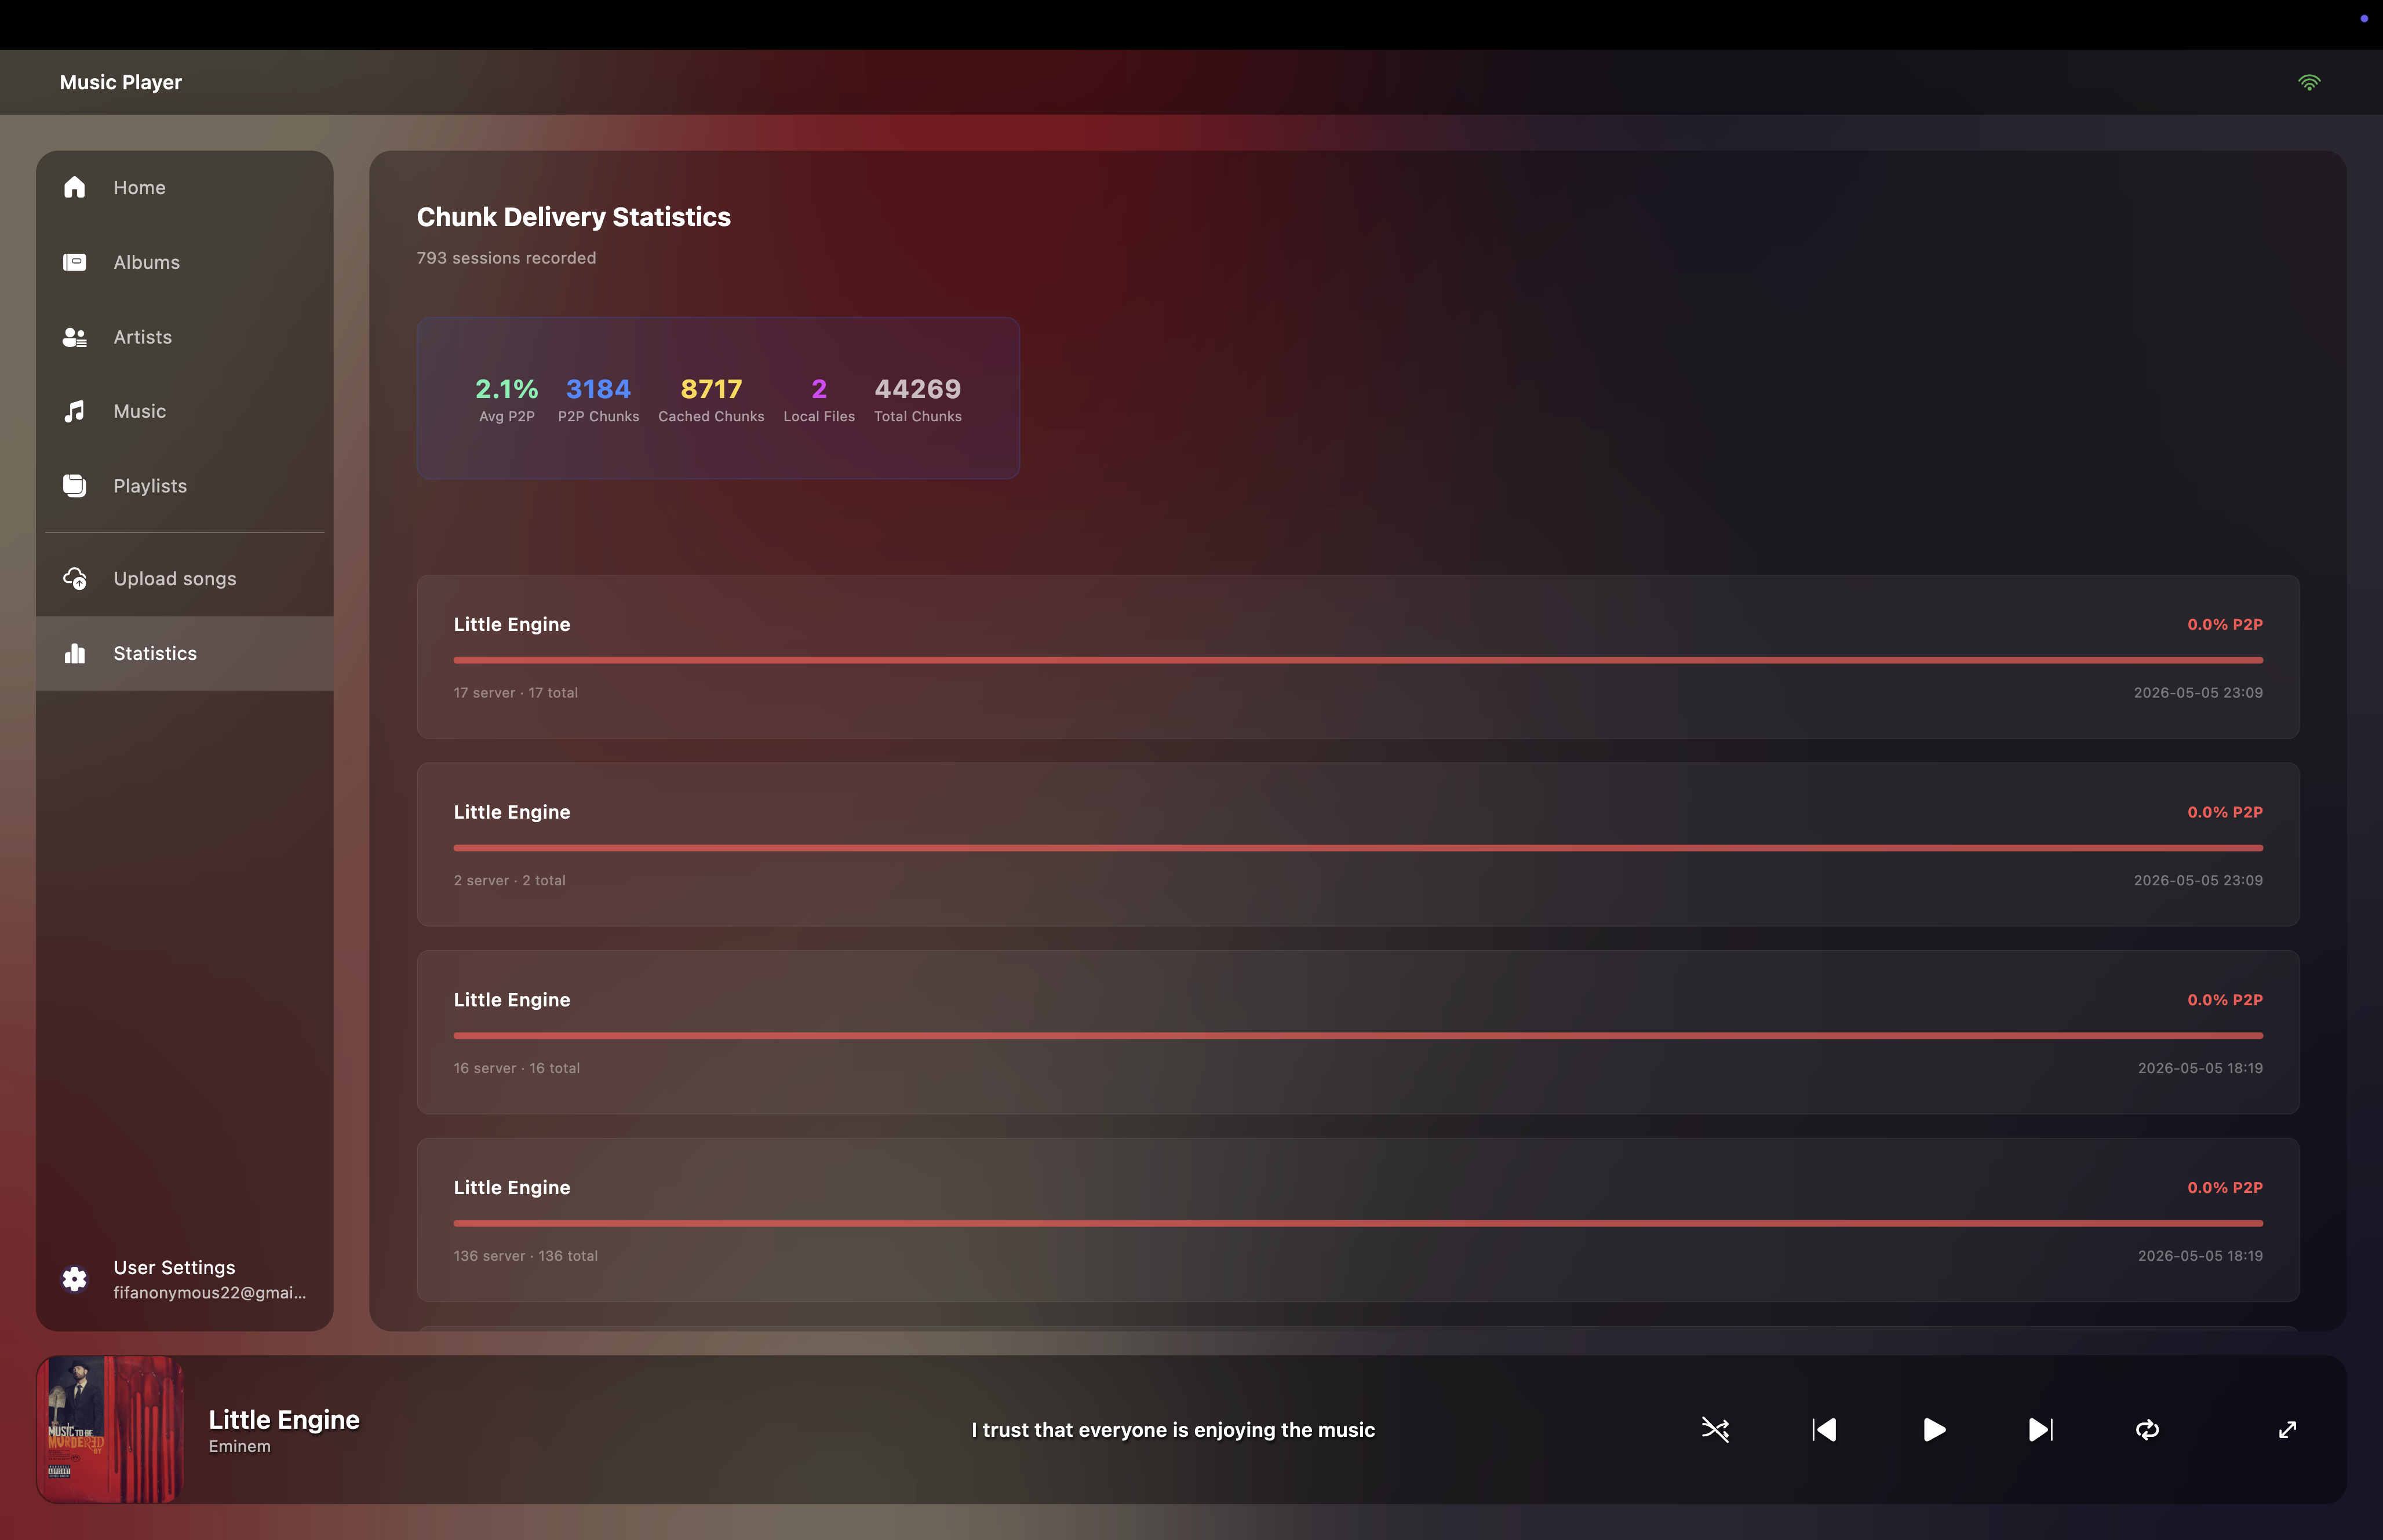
\includegraphics[width=\textwidth]{figures/screenshots/stats_screen.png}
\caption{Statistics screen after a streaming session, showing the aggregate offload card and the per-session breakdown.}
\label{fig:exec-stats}
\end{figure}

\par The relatively low average P2P share in Figure \ref{fig:exec-stats} is expected for this measurement setup, where most playback was performed by a single client with a warm local cache and no concurrent listener was available. Under more realistic deployment conditions, with several listeners playing the same song at the same time, the model in Chapter \ref{chap:ch2} predicts a much higher share, approaching the theoretical maximum.


\section{Mini User Manual}
\label{sec:user-manual}

\indent \par This section consolidates the steps above into a short reference. The numbers in parentheses point to the screenshots in Section \ref{sec:exec-f1}.

\begin{enumerate}
  \item Open the application and sign in with your email. The detailed authentication flow is described in Section \ref{subsec:auth}; once it completes, the home screen becomes visible (Figure \ref{fig:exec-home}).
  \item From the navigation drawer on the left, open the Music entry to reach the tracks view (Figure \ref{fig:exec-tracks}). You can also browse the catalogue through the Albums, Artists or Playlists entries.
  \item Click on a song. Playback starts almost immediately because the very first chunks are served by the origin server while the peer connections are still being negotiated. If other listeners are connected and have parts of the same song cached, the rest of the chunks are pulled directly from them; otherwise, the server keeps serving the song.
  \item Tap on the player bar at the bottom of the screen to open the now playing view (Figure \ref{fig:exec-now-playing}). From here you can pause, resume, skip, seek, toggle shuffle and repeat, and like the song.
  \item To upload your own songs, open the Upload songs entry in the drawer (Figures \ref{fig:screen-upload-empty} and \ref{fig:screen-upload-song}), pick the files from disk, and press Upload. The application will only transfer the chunks that the server does not already have.
  \item To control how much data the application uses for peer uploads, open the User Settings entry in the drawer (Figure \ref{fig:screen-settings}) and adjust the Peer Network dropdown together with the WiFi and Cellular data limits.
  \item To verify how much of your listening was served by peers versus by the server, open the Statistics entry in the drawer (Figure \ref{fig:exec-stats}). The aggregate card on top sums up every session, and the rows below it break each one down individually.
\end{enumerate}
